\section{Durchführung}
\label{sec:Durchführung}
Für den Aufbau des Experiments sind im wesentlichen ein Ultraschall Doppler-Generator, eine Ultraschallsonde mit einer Frequenz von $\SI{2}{\mega \hertz}$
und ein Rechner für die Datenaufnahme notwendig. Untersucht soll eine Strömungsröhre mit verschiedenen Innen-und Außendurchmessern werden. Als Flüssigkeit wird ein Gemisch aus Wasser, Glycerin und Glaskugeln verwendet.
Mit einer Zentrifugalpumpe kann die Strömungsgeschwindigkeit von $\SI{0}{rpm}$ bis $\SI{8600}{rpm}$ eingestellt werden. Die mit dem Echoskop gemessenen Daten werden mit dem Rechner
erfasst und ausgewertet.\\
Für die Untersuchung der Strömungsgeschwindigkeit und des Strömunsprofils werden Strömungsröhre mit Innendurchmessern von $\SI{7}{\milli\metre}$, $\SI{10}{\milli\metre}$ und $\SI{16}{\milli\metre}$ verwendet.
Für die Ankopplung der Ultraschallröhre an die Röhre werden Doppler-Prismen mit drei verschiedenen Einfallswinkeln verwendet(Siehe Abbildung \ref{fig:doppri}).
Es wurden jedoch die Einstellwinkel $\ang{15}$, $\ang{30}$ und $\ang{60}$ verwendet. Der Abstand zwischen Sonde und Flüssigkeit ist für alle drei Winkel gleich.
\begin{figure}
    \centering
    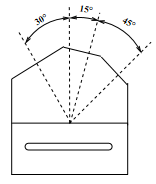
\includegraphics[scale=0.4]{pics/prisma.png}
    \caption{Doppler-Prisma mit 15°, 30° und 45° Einstellwinkeln \cite{}}
    \label{fig:doppri}
  \end{figure}
  Der Dopplerwinkel lässt sich mit
  \begin{equation}
    \alpha= \frac{pi}{2} - \arcsin\left(\sin \theta \frac{c_\text{L}}{c_\text{P}}\right)
      \label{eqn:wink}
  \end{equation}
  berechnen. Dabei ist $c_\text{L}=\SI{1800}{\metre\per\second}$ die Schallgeschwindigkeit in der Dopplerflüssigkeit und $c_\text{P}=\SI{2700}{\metre\per\second}$ die Schallgeschwindigkeit des Prismenmaterials. \\
  Zur Bestimmung der Strömungsgeschwindigkeit werden fünf verschiedene Flüssigkeitsgeschwindigkeiten als Funktion des Dopplerwinkels bestimmt. Die Messungen erfolgen an den drei verschiedenen Rohrdurchmessern.
Die Frequenzverschiebung kann direkt am Rechner abgelesen werden, sodass sich die Flüssigkeitsgeschwindigkeiten direkt berechnen lassen.\\
Um das Strömunsprofil der Dopplerflüssigkeit zu untersuchen, wird an dem $\SI{10}{\milli\metre}$ Schlauch gemessen. Es soll nur die Meßteiefe am Ultraschallgenerator variiert werden.
Dazu muss zuerst die Anfangstiefe bestimmt werden.Aufgrund der verschiedenen Schallgeschwindigkeiten in den Materialien muss eine kleine Zwischenrechnung durchgeführt werden.
Die Anfangstiefe kann danach auf den errechneten Wert $\SI{13}{\micro\second}$ gestellt werden. Nachdem die Zentrifugalpumpe auf $70 \si{\percent}$ der Maximalleistung gestellt wurde,
wird die Tiefe in $\SI{0.5}{\micro\second}$ erhöht, bis sie die maximale Tiefe $d=\SI{20}{\micro\second}$ erreicht. Es werden die Werte für die Frequenzverschiebung und die Streuintensität vom Rechner abgelesen.